%
% Complete documentation on the extended LaTeX markup used for Insight
% documentation is available in ``Documenting Insight'', which is part
% of the standard documentation for Insight.  It may be found online
% at:
%
%     http://www.itk.org/

\documentclass{InsightArticle}


%%%%%%%%%%%%%%%%%%%%%%%%%%%%%%%%%%%%%%%%%%%%%%%%%%%%%%%%%%%%%%%%%%
%
%  hyperref should be the last package to be loaded.
%
%%%%%%%%%%%%%%%%%%%%%%%%%%%%%%%%%%%%%%%%%%%%%%%%%%%%%%%%%%%%%%%%%%
\usepackage[dvips,
bookmarks,
bookmarksopen,
backref,
colorlinks,linkcolor={blue},citecolor={blue},urlcolor={blue},
]{hyperref}
% to be able to use options in graphics
\usepackage{graphicx}
% for pseudo code
\usepackage{listings}
% subfigures
\usepackage{subfigure}
\usepackage{pseudocode}


%  This is a template for Papers to the Insight Journal. 
%  It is comparable to a technical report format.

% The title should be descriptive enough for people to be able to find
% the relevant document. 
\title{Noise simulation}

% 
% NOTE: This is the last number of the "handle" URL that 
% The Insight Journal assigns to your paper as part of the
% submission process. Please replace the number "1338" with
% the actual handle number that you get assigned.
%
\newcommand{\IJhandlerIDnumber}{3158}

% Increment the release number whenever significant changes are made.
% The author and/or editor can define 'significant' however they like.
% \release{0.00}

% At minimum, give your name and an email address.  You can include a
% snail-mail address if you like.
\author{Ga\"etan Lehmann}
% \authoraddress{}

\begin{document}

%
% Add hyperlink to the web location and license of the paper.
% The argument of this command is the handler identifier given
% by the Insight Journal to this paper.
% 
\IJhandlefooter{\IJhandlerIDnumber}

\maketitle

\ifhtml
\chapter*{Front Matter\label{front}}
\fi


\begin{abstract}
\noindent
% The abstract should be a paragraph or two long, and describe the
% scope of the document.
Several kind of noise can be found in real images, mostly depending on the modality
of acquisition. It is often useful to be able to simulate that noise, for example
to test the behavior of an algorithm in the presence of a known amount of noise.

This contribution provides the filters to generate four kind of noise -- additive
gaussian, shot, speckle and salt and pepper -- as well as a PSNR calculator.
\end{abstract}

\IJhandlenote{\IJhandlerIDnumber}

\tableofcontents

\section{Noise types}

\subsection{Additive gaussian noise}

This is the most frequent kind of noise. It can be modeled as:
\begin{eqnarray}
\label{eq:gauss}
I = I_0 + N
\end{eqnarray}
where $I$ is the observed image, $I_0$ is the non-noisy image and $N$ is a normally distributed random
variable of mean $\mu$ and variance $\sigma^2$. The noise is independant of the pixel intensities.
\begin{eqnarray}
N \sim \mathcal{N}(\mu,\sigma^2)
\end{eqnarray}
$\mu$ is generally $0$.

Additive gaussian noise can be simulated with \code{itk::AdditiveGaussianNoiseImageFilter}. The mean
can be specified with \code{SetMean()} and the standard deviation with \code{SetStandardDeviation()}.
The mean defaults to $0$ and the standard deviation to $1$.

\begin{figure}[htbp]
\begin{center}
\subfigure[Input image]{\includegraphics[scale=0.6]{cthead1}}
\subfigure[Noisy image]{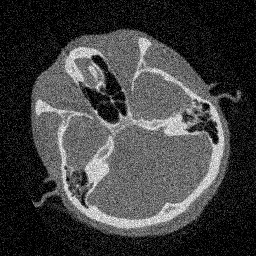
\includegraphics[scale=.6]{gauss}}
\subfigure[Generated noise]{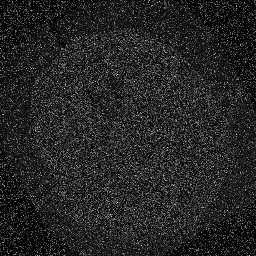
\includegraphics[scale=.6]{dgauss}}
\caption{(a) the input image. (b) image altered with additive gaussian noise with $\mu = 0$ and
$\sigma = 22.8$. (c) the generated noise extracted by computing the absolute difference between (a)
and (b). Note that the noise is {\em almost} independant of the pixel intensities -- the dark zones
show less noise because of the clipping of the negative values applied to the pixel intensities
during the simulation. The command line used was {\em ./gauss ../images/cthead1.tif gauss.png 22.8}.}
\end{center}
\end{figure}

\subsection{Shot noise}

Shot noise, also called Poisson noise or photon noise can be modeled as:
\begin{eqnarray}
\label{eq:shot}
I = N(I_0)
\end{eqnarray}
where $N(I_0)$ is a poisson distributed random variable of mean $I_0$. The noise is thus dependant on
the pixel intensities in the image.

Shot noise can be simulated with \code{itk::ShotNoiseImageFilter}. The intensities in the image can be
scaled by a user provided value to map the pixel value to the actual number of photon. The scaling
can be seen as the inverse of the gain used during the acquisition. The noisy signal is then scaled
back to its input intensity range.
\begin{eqnarray}
I = \frac{N(I_0 \times s)}{s}
\end{eqnarray}
where $s$ is the scale factor.

The scale factor can be set with \code{SetScale()}.

\begin{figure}[htbp]
\begin{center}
\subfigure[Input image]{\includegraphics[scale=0.6]{cthead1}}
\subfigure[Noisy image]{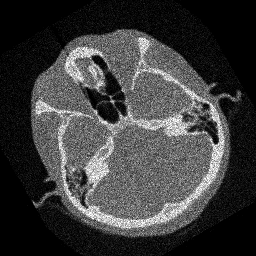
\includegraphics[scale=.6]{shot}}
\subfigure[Generated noise]{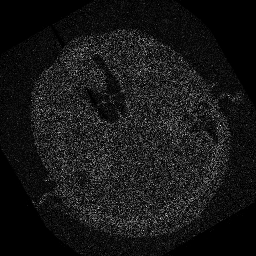
\includegraphics[scale=.6]{dshot}}
\caption{(a) the input image. (b) image altered with shot noise with $s = 0.15$.
(c) the generated noise extracted by computing the absolute difference between (a)
and (b). Note that the noise is dependant of the pixel intensities -- a strong signal leads to a
strong noise. The command line used was {\em ./shot ../images/cthead1.tif shot.png 0.15}.}
\end{center}
\end{figure}

The poisson distributed variable is computed by using the code

\begin{pseudocode}{poissonDistributedVariable}{\lambda}
k \GETS 0 \\
p \GETS 1 \\
\REPEAT
\BEGIN
  k \GETS k + 1 \\
  p \GETS p * \CALL{U}{} \\
\END
\UNTIL{p > e^{-\lambda}} \\
\RETURN k
\end{pseudocode}

where $U()$ provides a uniformly distributed random variable in the interval $[0, 1]$.

This algorithm is very inefficient for large value of $\lambda$ though. Fortunately, the poisson
distribution can be accurately approximated by a Gaussian distribution $\lambda$ of mean and
variance $\lambda$ when $\lambda$ is large enough. This leads to this faster algorithm:

\begin{pseudocode}{approximatedPoissonDistributedVariable}{\lambda}
\IF \lambda \le 50
\THEN
  \RETURN{\CALL{poissonDistributedVariable}{\lambda}}
\ELSE
  \RETURN{\lambda + \sqrt{\lambda} \times \CALL{N}{}}
\end{pseudocode}

where $N()$ produce a normally distribution variable of mean $0$ and variance $1$.


\subsection{Speckle noise}

Speckle noise is also called multiplicative noise. It can be modeled as:

\begin{eqnarray}
\label{eq:speckle}
I = I_0 * G
\end{eqnarray}
where G is a is a gamma distributed random variable of mean $1$ and variance proportional to
the noise level.

\begin{eqnarray}
G \sim \Gamma(\frac{1}{\sigma^2},\sigma^2)
\end{eqnarray}

Speckle noise can be simulated with \code{itk::SpeckleNoiseImageFilter}. The standard deviation
of the noise can be set with \code{SetStandardDeviation()} and defaults to $1$.

\begin{figure}[htbp]
\begin{center}
\subfigure[Input image]{\includegraphics[scale=0.6]{cthead1}}
\subfigure[Noisy image]{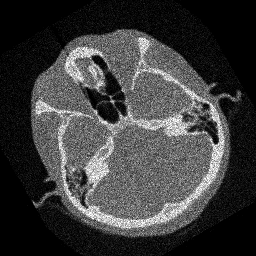
\includegraphics[scale=.6]{shot}}
\subfigure[Generated noise]{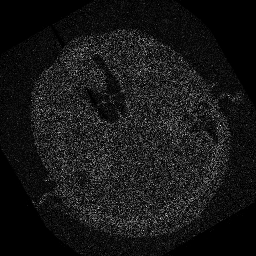
\includegraphics[scale=.6]{dshot}}
\caption{(a) the input image. (b) image altered with speckle noise with $\sigma = 0.24$.
(c) the generated noise extracted by computing the absolute difference between (a)
and (b). Note that the noise is dependant of the pixel intensities -- a strong signal leads to a
strong noise. The command line used was {\em ./speckle ../images/cthead1.tif speckle.png 0.24}.}
\end{center}
\end{figure}

The gamma distributed random variable is a bit more difficult to compute than what is done in the
previous cases.

\begin{pseudocode}{gammaDistributedVariable}{k, \theta}
\delta \GETS {k} \\
v_0 \GETS \frac{e}{e+\delta} \\
\REPEAT
\BEGIN
  v_1 \GETS \CALL{U}{}, v_2 \GETS \CALL{U}{}, v_3 \GETS \CALL{U}{} \\
  \IF v_1 \leq v_0
  \THEN
    \BEGIN
    \xi \GETS v_2^{1/\delta} \\
    \nu \GETS v_3 \xi^{\delta-1} \\
    \END
  \ELSE
    \BEGIN
    \xi \GETS 1 - ln v_2 \\
    \nu \GETS v_3 e^{-\xi} \\
  \END
\END
\UNTIL{\nu > e^{-\xi} \xi^{\delta-1}} \\
\RETURN{\theta \left(\xi - \underset{i=1}{\overset{[k]}{\sum}} ln \CALL{U}{}\right)}
\end{pseudocode}

where $U()$ produce a uniformaly distributed variable on the lower open range $(0, 1]$, $[k]$ is the
integral value of $k$ and ${k}$ is the decimal value of $k$.

\subsection{Salt and pepper noise}

Salt and pepper noise is a special kind of impulse noise where the value of the noise is either
the maximum possible value in the image or its minimum. It can be modeled as:
\begin{eqnarray}
\label{eq:sp}
I = 
\begin{cases} 
  M,  & \text{if}~ U < p/2 \\
  m,  & \text{if}~ U > 1 - p/2 \\
  I_0,& \text{if}~ p/2 \geq U \leq 1 - p/2 \\
\end{cases}
\end{eqnarray}

where $p$ is the probability of apparition of the noise, $U$ is a uniformally distributed
random variable on the range $[0, 1]$, $M$ is the greatest possible pixel value and $m$ the
smallest possible pixel value.

Salt and pepper noise can be simulated with \code{itk::SaltAndPepperNoiseImageFilter}. The probability
of the noise can be set with \code{SetProbability()} and defaults to $0.01$.

\begin{figure}[htbp]
\begin{center}
\subfigure[Input image]{\includegraphics[scale=0.6]{cthead1}}
\subfigure[Noisy image]{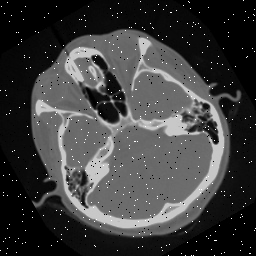
\includegraphics[scale=.6]{sp}}
\subfigure[Generated noise]{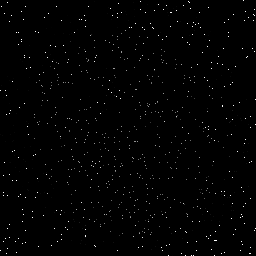
\includegraphics[scale=.6]{dsp}}
\caption{(a) the input image. (b) image altered with salt and pepper noise with $p = 0.016$.
(c) the generated noise extracted by computing the absolute difference between (a)
and (b). Note that the noise is independant of the pixel intensities.
The command line used was {\em ./sp ../images/cthead1.tif sp.png 0.016}.}
\end{center}
\end{figure}

\section{Peak signal-to-noise ratio}

The peak signal-to-noise ratio (PSNR) is a measure of degradation of the image quality.
It is computed as

\begin{eqnarray}
PSNR = 10 \cdot log_{10}\left(\frac{M^2 \cdot N}{\underset{p \in D}{\sum} (I_0[p]-I[p])^2}\right)
\end{eqnarray}

where $D$ is the domain of definition of the image $I_0$ and $I$, $N$ is the number of pixel in $D$,
and $M$ is the maximum possible value in $I$.

All the images degraded with noise in this article have a PSNR around $22.1$.

\section{Wrapping}

All the new filters have been wrapped using WrapITK.

\section{Development details}

\code{itk::MersenneTwisterRandomVariateGenerator} has been modified to produce a thread safe
implementation called \code{itk::ThreadSafeMersenneTwisterRandomVariateGenerator}. It should be
possible to fix the non thread safety in the original class, but the implication on the testing
framework and the backward compatibility are beyond the scope of this contribution.

The filters are {\em not} implemented as subclasses of \code{itk::UnaryFunctorImageFilter}
because each thread must have its own random generator. They are implemented as subclasses
of \code{itk::InPlaceImageFilter} to be able to run the noise addition in place. All the
filters are multithreaded.

Due to the difficulty of testing a random behavior, no test is provided.

A development version is available in a darcs repository at
\url{http://mima2.jouy.inra.fr/darcs/contrib-itk/noise/}.

\section{Conclusion}

\section{Acknowledgments}

Unlike most of my previous contributions, this work has {\em not} been supported by
the french National Institute for Agricultural Research (INRA) -- my employer.
I'd like to thanks the INRA anyway, and more specifically the MIMA2 facility, to
have provided the computer ressources used for this work. 

\section{References}

Most of the informations used in this article are coming from wikipedia.

\url{http://en.wikipedia.org/wiki/Additive_white_Gaussian_noise}

\url{http://en.wikipedia.org/wiki/Shot_noise}

\url{http://en.wikipedia.org/wiki/Poisson_distribution}

\url{http://en.wikipedia.org/wiki/Speckle_noise}

\url{http://en.wikipedia.org/wiki/Gamma_distribution#Generating_gamma-distributed_random_variables}

\url{http://www.ceremade.dauphine.fr/~peyre/numerical-tour/tours/denoising_data_dependent}

\url{http://en.wikipedia.org/wiki/PSNR}



\end{document}

